\documentclass[../entwurf.tex]{subfiles}

\begin{document}

% Titel und Inhaltsübersicht
\maketitle
\tableofcontents

\clearpage
\section{Praeambel}
Ziel des Entwurfsdokuments ist die Systemarchitektur der App 'Karl' darzustellen. Hierfür haben wir UML-Klassendiagramme innerhalb einer Model-View-ViewModel Architektur verwendet.

	\begin{center}
		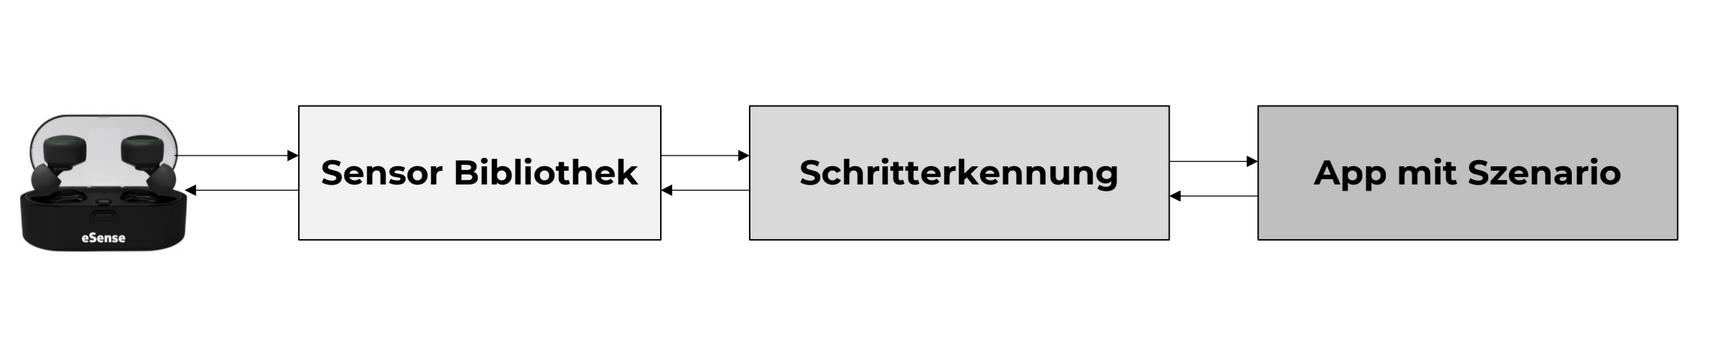
\includegraphics[page=1,width=350pt,keepaspectratio]{../graphics/Praeambel/YHB_Project_Pic.png}
		\textit{Spezifikation der Earable-Plattform }
	\end{center}

Zu jeder Schicht, Klasse, Attribut und Methode sind kurze Beschreibungen vorhanden. Hinzu kommen Sequenzdiagramme, um Abläufe von User-Interaktonen, wie zum Beispiel das Verbinden mit den Earables, zu veranschaulichen.

\end{document}
